% Options for packages loaded elsewhere
\PassOptionsToPackage{unicode}{hyperref}
\PassOptionsToPackage{hyphens}{url}
%
\documentclass[
]{article}
\usepackage{lmodern}
\usepackage{amssymb,amsmath}
\usepackage{ifxetex,ifluatex}
\ifnum 0\ifxetex 1\fi\ifluatex 1\fi=0 % if pdftex
  \usepackage[T1]{fontenc}
  \usepackage[utf8]{inputenc}
  \usepackage{textcomp} % provide euro and other symbols
\else % if luatex or xetex
  \usepackage{unicode-math}
  \defaultfontfeatures{Scale=MatchLowercase}
  \defaultfontfeatures[\rmfamily]{Ligatures=TeX,Scale=1}
\fi
% Use upquote if available, for straight quotes in verbatim environments
\IfFileExists{upquote.sty}{\usepackage{upquote}}{}
\IfFileExists{microtype.sty}{% use microtype if available
  \usepackage[]{microtype}
  \UseMicrotypeSet[protrusion]{basicmath} % disable protrusion for tt fonts
}{}
\makeatletter
\@ifundefined{KOMAClassName}{% if non-KOMA class
  \IfFileExists{parskip.sty}{%
    \usepackage{parskip}
  }{% else
    \setlength{\parindent}{0pt}
    \setlength{\parskip}{6pt plus 2pt minus 1pt}}
}{% if KOMA class
  \KOMAoptions{parskip=half}}
\makeatother
\usepackage{xcolor}
\IfFileExists{xurl.sty}{\usepackage{xurl}}{} % add URL line breaks if available
\IfFileExists{bookmark.sty}{\usepackage{bookmark}}{\usepackage{hyperref}}
\hypersetup{
  hidelinks,
  pdfcreator={LaTeX via pandoc}}
\urlstyle{same} % disable monospaced font for URLs
\usepackage{color}
\usepackage{fancyvrb}
\newcommand{\VerbBar}{|}
\newcommand{\VERB}{\Verb[commandchars=\\\{\}]}
\DefineVerbatimEnvironment{Highlighting}{Verbatim}{commandchars=\\\{\}}
% Add ',fontsize=\small' for more characters per line
\newenvironment{Shaded}{}{}
\newcommand{\AlertTok}[1]{\textcolor[rgb]{1.00,0.00,0.00}{\textbf{#1}}}
\newcommand{\AnnotationTok}[1]{\textcolor[rgb]{0.38,0.63,0.69}{\textbf{\textit{#1}}}}
\newcommand{\AttributeTok}[1]{\textcolor[rgb]{0.49,0.56,0.16}{#1}}
\newcommand{\BaseNTok}[1]{\textcolor[rgb]{0.25,0.63,0.44}{#1}}
\newcommand{\BuiltInTok}[1]{#1}
\newcommand{\CharTok}[1]{\textcolor[rgb]{0.25,0.44,0.63}{#1}}
\newcommand{\CommentTok}[1]{\textcolor[rgb]{0.38,0.63,0.69}{\textit{#1}}}
\newcommand{\CommentVarTok}[1]{\textcolor[rgb]{0.38,0.63,0.69}{\textbf{\textit{#1}}}}
\newcommand{\ConstantTok}[1]{\textcolor[rgb]{0.53,0.00,0.00}{#1}}
\newcommand{\ControlFlowTok}[1]{\textcolor[rgb]{0.00,0.44,0.13}{\textbf{#1}}}
\newcommand{\DataTypeTok}[1]{\textcolor[rgb]{0.56,0.13,0.00}{#1}}
\newcommand{\DecValTok}[1]{\textcolor[rgb]{0.25,0.63,0.44}{#1}}
\newcommand{\DocumentationTok}[1]{\textcolor[rgb]{0.73,0.13,0.13}{\textit{#1}}}
\newcommand{\ErrorTok}[1]{\textcolor[rgb]{1.00,0.00,0.00}{\textbf{#1}}}
\newcommand{\ExtensionTok}[1]{#1}
\newcommand{\FloatTok}[1]{\textcolor[rgb]{0.25,0.63,0.44}{#1}}
\newcommand{\FunctionTok}[1]{\textcolor[rgb]{0.02,0.16,0.49}{#1}}
\newcommand{\ImportTok}[1]{#1}
\newcommand{\InformationTok}[1]{\textcolor[rgb]{0.38,0.63,0.69}{\textbf{\textit{#1}}}}
\newcommand{\KeywordTok}[1]{\textcolor[rgb]{0.00,0.44,0.13}{\textbf{#1}}}
\newcommand{\NormalTok}[1]{#1}
\newcommand{\OperatorTok}[1]{\textcolor[rgb]{0.40,0.40,0.40}{#1}}
\newcommand{\OtherTok}[1]{\textcolor[rgb]{0.00,0.44,0.13}{#1}}
\newcommand{\PreprocessorTok}[1]{\textcolor[rgb]{0.74,0.48,0.00}{#1}}
\newcommand{\RegionMarkerTok}[1]{#1}
\newcommand{\SpecialCharTok}[1]{\textcolor[rgb]{0.25,0.44,0.63}{#1}}
\newcommand{\SpecialStringTok}[1]{\textcolor[rgb]{0.73,0.40,0.53}{#1}}
\newcommand{\StringTok}[1]{\textcolor[rgb]{0.25,0.44,0.63}{#1}}
\newcommand{\VariableTok}[1]{\textcolor[rgb]{0.10,0.09,0.49}{#1}}
\newcommand{\VerbatimStringTok}[1]{\textcolor[rgb]{0.25,0.44,0.63}{#1}}
\newcommand{\WarningTok}[1]{\textcolor[rgb]{0.38,0.63,0.69}{\textbf{\textit{#1}}}}
\usepackage{graphicx,grffile}
\makeatletter
\def\maxwidth{\ifdim\Gin@nat@width>\linewidth\linewidth\else\Gin@nat@width\fi}
\def\maxheight{\ifdim\Gin@nat@height>\textheight\textheight\else\Gin@nat@height\fi}
\makeatother
% Scale images if necessary, so that they will not overflow the page
% margins by default, and it is still possible to overwrite the defaults
% using explicit options in \includegraphics[width, height, ...]{}
\setkeys{Gin}{width=\maxwidth,height=\maxheight,keepaspectratio}
% Set default figure placement to htbp
\makeatletter
\def\fps@figure{htbp}
\makeatother
\setlength{\emergencystretch}{3em} % prevent overfull lines
\providecommand{\tightlist}{%
  \setlength{\itemsep}{0pt}\setlength{\parskip}{0pt}}
\setcounter{secnumdepth}{-\maxdimen} % remove section numbering

\date{}

\begin{document}

\hypertarget{header-n0}{%
\section{SE-344}\label{header-n0}}

\hypertarget{header-n2}{%
\subsection{Assignment \#2 Report}\label{header-n2}}

\begin{itemize}
\item
  姓名:于喜千
\item
  学号:\texttt{517030910168}
\item
  任务:Assignment \#2
\end{itemize}

\hypertarget{header-n10}{%
\subsubsection{细节描述}\label{header-n10}}

\hypertarget{header-n11}{%
\paragraph{第一部分:搭建 OpenGL 编程环境}\label{header-n11}}

\hypertarget{header-n12}{%
\subparagraph{环境设定}\label{header-n12}}

\begin{itemize}
\item
  Windows 10 x64 LTSC 1809 (\texttt{17763.737})
\item
  Visual Studio 2019 Community (\texttt{16.2.4})
\item
  FreeGLUT
\end{itemize}

此处,比照 Assignment \#1 中的环境设定办理。

\hypertarget{header-n21}{%
\paragraph{第二部分:数据处理}\label{header-n21}}

由于本次 Assignment 中的三角形数据来自 \texttt{overlapping.tri} 和
\texttt{intersecting.tri},因此我们首先需要实现三角形数据的读取。

\hypertarget{header-n23}{%
\subparagraph{标准库使用}\label{header-n23}}

这里,主要利用了 C++ 中的 \texttt{\textless{}fstream\textgreater{}} 和
\texttt{\textless{}iostream\textgreater{}} 标准库来实现文件数据的读取。

\hypertarget{header-n25}{%
\subparagraph{数据格式}\label{header-n25}}

在作业提供的 \texttt{.tri} 文件中,包含由不定数量的空格符及
\texttt{\textquotesingle{}\textbackslash{}n\textquotesingle{}}
分隔的数字;这些数字依次代表了三角形每个顶点的 x、y、z
坐标位置(有符号整数)及 R、G、B 颜色分量(0 ~ 1 之间的浮点数)。

文件以 \texttt{\textquotesingle{}\textbackslash{}n\textquotesingle{}} +
EOF 结束。

\hypertarget{header-n28}{%
\subparagraph{程序结构}\label{header-n28}}

相关文件包括 \texttt{Triangle.hpp}、\texttt{Reader.h}、和
\texttt{Reader.cpp}。

在 \texttt{Triangle.hpp} 中,定义着 \texttt{TrianglePoint} 和
\texttt{Triangle}
两个类;他们用于结构化地描述三角形的顶点位置及顶点颜色。同时,提供了默认的无参构造函数及完整构造函数,方便各种形式的调用;同时在构造时还对
R、G、B 颜色分量进行了范围检测和归一化纠错,减少错误调用的可能性。

在 \texttt{Reader.cpp} + \texttt{Reader.h} 两个文件中,定义了一个名为
\texttt{readTriangle}
的参数;它可以通过提供文件名作为参数来读取所有满足上述条件的
\texttt{.tri} 文件,并将其放置在
\texttt{vector\textless{}Triangle\textgreater{}}
中并返回。这就意味着我们可以在随后的 Phases
中复用这个函数,减少重复工作,提高程序效能。

\hypertarget{header-n32}{%
\subparagraph{执行结果}\label{header-n32}}

通过断点调试方法,发现程序可以成功处理 \texttt{overlapping.tri} 和
\texttt{intersecting.tri} 两个 \texttt{.tri} 文件,并能正确生成
\texttt{Triangle} 对象。

\hypertarget{header-n34}{%
\paragraph{第三部分:三角形绘制}\label{header-n34}}

\hypertarget{header-n353}{%
\subparagraph{程序结构}\label{header-n353}}

这一部分的代码更改主要在 \texttt{main.cpp}
的渲染部分。另外,扫描线算法的实现位于 \texttt{DepthChecker.hpp} 中。

首先,我们引入 \texttt{Triangle.hpp} 及 \texttt{Reader.h}
头文件来读入所需的文件。

\hypertarget{header-n36}{%
\subparagraph{读取数据}\label{header-n36}}

\begin{Shaded}
\begin{Highlighting}[]
\KeywordTok{auto}\NormalTok{ triangles = readTriangle(}\StringTok{"./overlapping.tri"}\NormalTok{);}
\CommentTok{/* 'triangles' type: std::vector<Triangles> */}
\end{Highlighting}
\end{Shaded}

由于除错调试时的 \texttt{.tri}
文件路径和实际运行时的路径有出入,因此为了保证程序灵活性,采用运行时指定文件路径的做法,如此:

\begin{Shaded}
\begin{Highlighting}[]
\BuiltInTok{std::}\NormalTok{cin >> path;}
\KeywordTok{auto}\NormalTok{ triangles = readTriangle(path);}
\end{Highlighting}
\end{Shaded}

\hypertarget{header-n46}{%
\subparagraph{绘制三角形}\label{header-n46}}

为了减少代码绘制时产生的问题,这里复用了上一次的视角旋转代码来实现视角的改变。

同样,绘制图形的代码在 \texttt{onRender()} 函数中实现。

启用深度检测

在 \texttt{main} 函数中,我们使用下列方法来启用深度检测:

\begin{Shaded}
\begin{Highlighting}[]
\CommentTok{// 设置深度缓存}
\NormalTok{glClearDepth(}\FloatTok{1.0}\NormalTok{);}

\CommentTok{// 启用深度测试}
\NormalTok{glEnable(GL_DEPTH_TEST);}

\CommentTok{// 所作深度测试的类型}
\NormalTok{glDepthFunc(GL_LEQUAL);}

\CommentTok{// 启用平滑}
\NormalTok{glShadeModel(GL_SMOOTH);}
\end{Highlighting}
\end{Shaded}

关键方法为 \texttt{glEnable(GL\_DEPTH\_TEST)},该函数启用了 GLUT
提供的深度测试。

留意到我们需要使用重心差值渐变来绘制三角形,因此我们调用
\texttt{glShadeModel(GL\_SMOOTH)} 函数。

而 \texttt{glDepthFunc(...)}
函数可以指定进行深度测试的类型。可以使用的参数包括:

\begin{itemize}
\item
  \texttt{GL\_NEVER}, 总是不通过(输入的深度值不取代参考值)
\item
  \texttt{GL\_LESS}, 如果输入的深度值小于参考值,则通过
\item
  \texttt{GL\_EQUAL}, 如果输入的深度值等于参考值,则通过
\item
  \texttt{GL\_LEQUAL}, 如果输入的深度值小于或等于参考值,则通过
\item
  \texttt{GL\_GREATER}, 如果输入的深度值大于参考值,则通过
\item
  \texttt{GL\_NOTEQUAL}, 如果输入的深度值不等于参考值,则通过
\item
  \texttt{GL\_GEQUAL}, 如果输入的深度值大于或等于参考值,则通过
\item
  \texttt{GL\_ALWAYS}, 总是通过(输入的深度值取代参考值)
\end{itemize}

(Refs: glDepthFunc - OpenGL 4 Reference Pages)

清除缓存

由于开启了深度检测,因此我们在每次开始渲染时,不仅要清除像素缓存
Bit(\texttt{GL\_COLOR\_BUFFER\_BIT}),同时还要清除深度缓存
Bit(\texttt{GL\_DEPTH\_BUFFER\_BIT})。

\begin{Shaded}
\begin{Highlighting}[]
\NormalTok{glClear(GL_COLOR_BUFFER_BIT | GL_DEPTH_BUFFER_BIT);}
\end{Highlighting}
\end{Shaded}

绘制三角形

因为我们已经得到了 \texttt{Triangle} 数组,因此只需要使用
\texttt{glBegin(GL\_TRIANGLES)} 来绘制就好了。

在 \texttt{glBegin} 和 \texttt{glEnd} 之间,连续调用 \texttt{glColor3d}
和 \texttt{glVertex3d} 来绘制不同颜色的顶点。

绘制参考线

\begin{Shaded}
\begin{Highlighting}[]
\NormalTok{glColor3d(}\FloatTok{0.6}\NormalTok{, }\FloatTok{0.6}\NormalTok{, }\FloatTok{0.7}\NormalTok{);}
\ControlFlowTok{for}\NormalTok{ (}\DataTypeTok{float}\NormalTok{ i = -}\DecValTok{50}\NormalTok{; i <= }\DecValTok{50}\NormalTok{; i += }\FloatTok{0.2}\BuiltInTok{f}\NormalTok{)}
\NormalTok{\{}
	\CommentTok{/** 绘制线 */}
\NormalTok{	glBegin(GL_LINES);}

	\CommentTok{/** x 轴方向 */}
\NormalTok{	glVertex3f(-}\DecValTok{50}\NormalTok{, }\DecValTok{0}\NormalTok{, i);}
\NormalTok{	glVertex3f(}\DecValTok{50}\NormalTok{, }\DecValTok{0}\NormalTok{, i);}

	\CommentTok{/** z 轴方向 */}
\NormalTok{	glVertex3f(i, }\DecValTok{0}\NormalTok{, -}\DecValTok{50}\NormalTok{);}
\NormalTok{	glVertex3f(i, }\DecValTok{0}\NormalTok{, }\DecValTok{50}\NormalTok{);}

\NormalTok{	glEnd();}
\NormalTok{\}}
\end{Highlighting}
\end{Shaded}

为了保证空间视觉观看体验,因此我们在 xOz
平面上绘制一系列的灰色网格来帮助我们观察。

\hypertarget{header-n167}{%
\subparagraph{观察结果}\label{header-n167}}

根据程序读取 \texttt{overlapping.tri} 和 \texttt{intersecting.tri}
的结果来看,可以看出 OpenGL 提供的深度检测算法表现优异,运行高效。

\begin{figure}
\centering
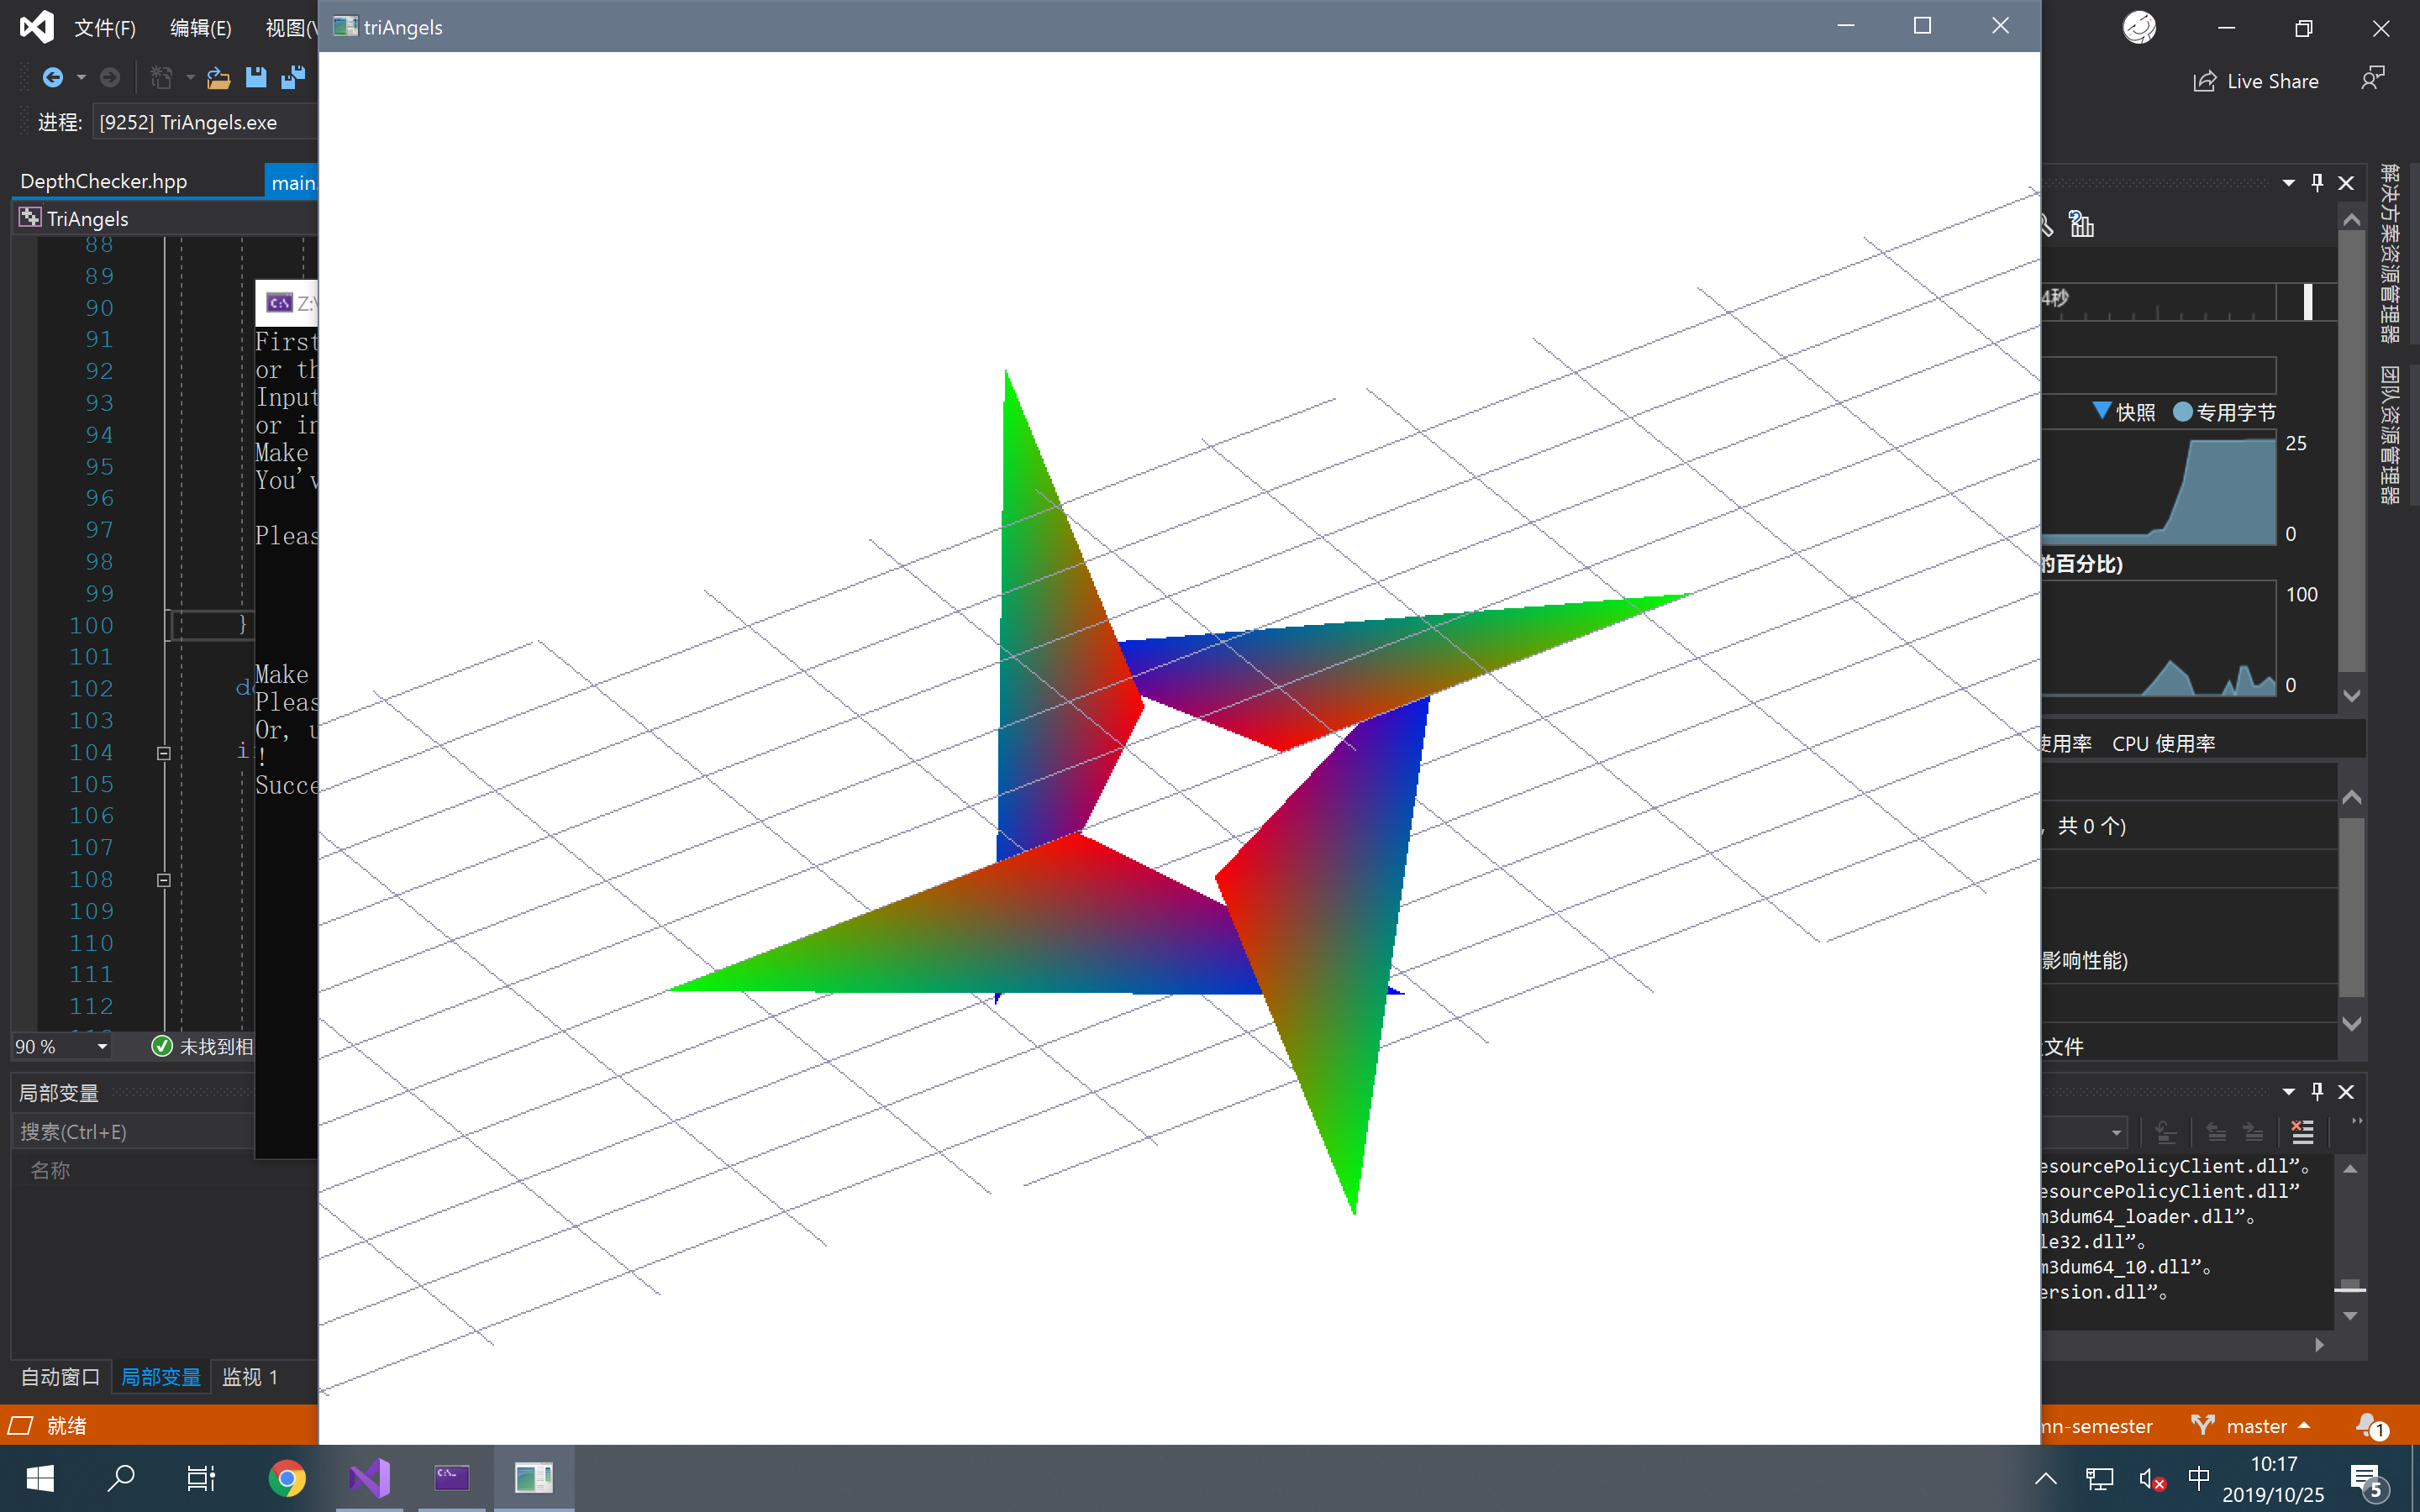
\includegraphics{/Users/yue/Documents/GitHub/2019-2020-autumn-semester/SE-344/submissions/ass2/screenshots/img.001.png}
\caption{}
\end{figure}

\begin{quote}
「\texttt{overlapping.tri}」的渲染结果,使用随附的深度检测算法
\end{quote}

\begin{figure}
\centering
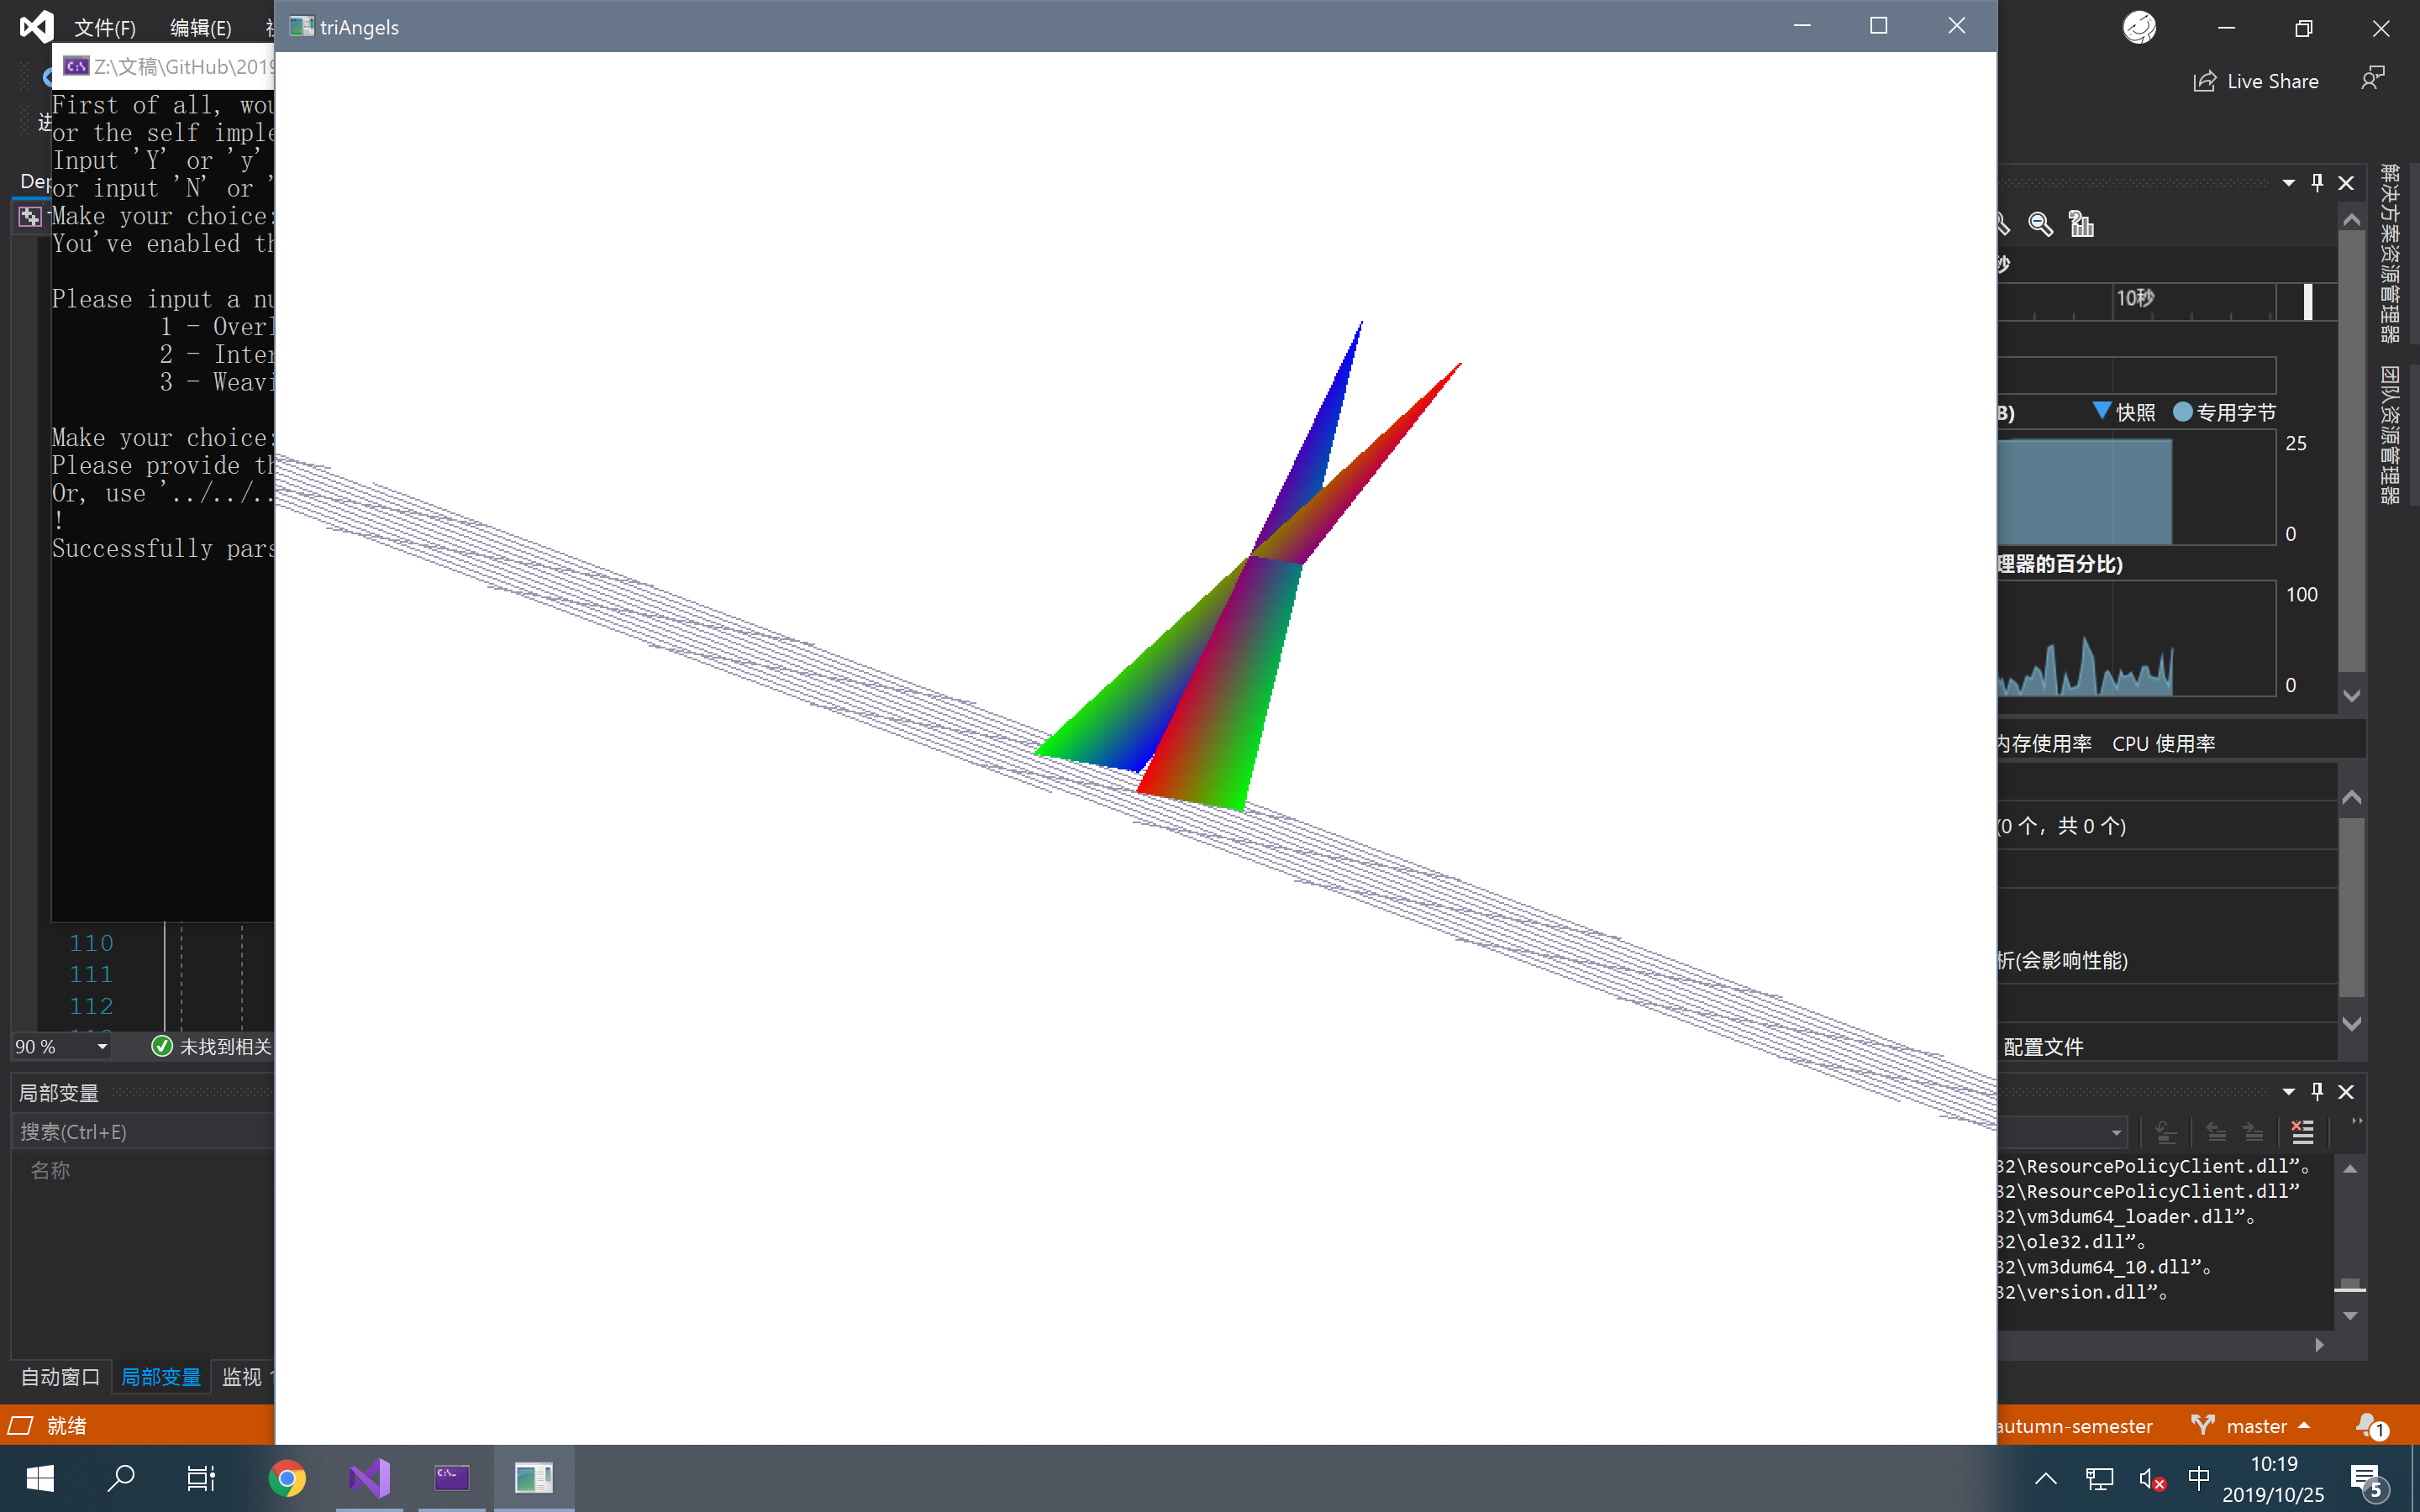
\includegraphics{/Users/yue/Documents/GitHub/2019-2020-autumn-semester/SE-344/submissions/ass2/screenshots/img.002.png}
\caption{}
\end{figure}

\begin{quote}
「\texttt{intersecting.tri}」的渲染结果,使用随附的深度检测算法
\end{quote}

\hypertarget{header-n187}{%
\paragraph{第四部分:扫描线算法}\label{header-n187}}

\hypertarget{header-n194}{%
\subparagraph{兼容修改}\label{header-n194}}

为了保证在实现扫描线算法的过程中,不要破坏上面已经完成的代码,这里新增了一个名为
\texttt{useDefaultDepthCheck}
的开关;程序运行起始会询问是否打开这一开关。

\hypertarget{header-n192}{%
\subparagraph{思路说明}\label{header-n192}}

为了简便起见,也因为图形较为简单,这里使用了最简单的思路:

\begin{enumerate}
\def\labelenumi{\arabic{enumi}.}
\item
  在 \(xOy\)
  平面内遍历所有点,判断其是否和三角形存在交点;映射完成后跳转到第 5
  步。
\item
  如果不存在交点,则忽略该点,回到第 1 步;
\item
  若存在唯一交点,则插值计算该交点的 \(z\) 坐标,并将 \((x, y, z)\)
  加入点映射表,回到第 1 步;
\item
  若存在多于 1
  个交点,则分别计算不同三角形的插值坐标,并比较采用其中最大的 \(z\)
  值,将其加入映射表;回到第 1 步;
\item
  从映射表中抽离出一个点集并返回给渲染器进行绘制。
\end{enumerate}

\hypertarget{header-n229}{%
\subparagraph{数学分析}\label{header-n229}}

这里存在两个数学问题:

一是如何判断与 \(z\) 轴平行的直线 \(x = x_0, y = y_0\) 是否穿过三角形;

二是如果穿过三角形,如何计算这条直线和三角形的交点坐标;

三是已知交点坐标,如何确定交点的 R、G、B 分量。

我们分别来进行分析。

相交判定

由于我们的渲染方向固定(沿着 \(z\)
轴向负方向观察),因此可以将三角形投影到 \(xOy\) 平面上进行计算。

于是问题可以抽象化为:已知平面 \(xOy\) 上四点
\(A\)、\(B\)、\(C\)、\(P\),判断点 P 是否在 \(A\)、\(B\)、\(C\)
构成的三角形内部。

这是一个简单的平面几何题。

要判断点是否在三角形内部,我们首先简化到判断点是否在一个方向向量的一侧。

而判断一个点是否在一个方向向量的一侧(左侧或右侧),我们可以采用差积(符号为
\(\times\))进行计算。

设已知的方向向量为 \(\overrightarrow{AB}\),要判断的点为
\(P\),则我们只需要判断向量 \(\overrightarrow{AB}\) 和
\(\overrightarrow{AP}\) 差积的符号即可。

当 \(P\) 在 \(\overrightarrow{AB}\)
左侧时,\(\overrightarrow{AB} \times \overrightarrow{AP}\)
应为正(根据右手螺旋法则);反之则在其右侧。

那么拓展到整个三角形,当点 \(P\) 同时在
\(\overrightarrow{AB}\)、\(\overrightarrow{BC}\)、\(\overrightarrow{CA}\)
的同侧时,即可判断其在三角形内部了。

\begin{quote}
\texttt{DepthChecker.hpp} 中的 \texttt{inTriangle} 函数实现了上述算法。
\end{quote}

交点计算

根据立体几何知识,不共线三点能确定一个平面。因此我们首先根据公式组

\[\left\{
\begin{aligned}
a & = & (p_{2_y} - p_{1_y}) \times (p_{3_z} - p_{1_z}) - (p_{2_z} - p_{1_z}) \times (p_{3_y} - p_{1_y}) \\
b & = & (p_{2_z} - p_{1_z}) \times (p_{3_x} - p_{1_x}) - (p_{2_x} - p_{1_x}) \times (p_{3_z} - p_{1_z}) \\
c & = & (p_{2_x} - p_{1_x}) \times (p_{3_y} - p_{1_y}) - (p_{2_y} - p_{1_y}) \times (p_{3_x} - p_{1_x}) \\
d & = &  - (a \times p_{1_x} + b \times p_{1_y} + c \times p_{1_z})
\end{aligned}
\right.\]

解出三点确定的平面公式 \(ax + by + cx + d = 0\)。

之后,我们将已知的射线 \(x = x_0, y = y_0\) 代入即可求出交点
\((x_0, y_0, z_0)\)。

\begin{quote}
\texttt{Triangle.hpp} 中的成员方法 \texttt{getPanelEquation}
实现了上述算法。
\end{quote}

颜色确定

这是一个比较麻烦的算法,主要原因是为了保证效果和原始图像的统一性,必须使用和原图相似的重心差值算法来进行颜色填充。

考虑到三角形是个平面图形,投影不会改变其插值性质;因此直接将其向观察面
\(xOy\) 上投影并计算颜色。

而计算颜色分量,本质上是计算三角形三个顶点的颜色决定权重;即每个点对于目标点具有多大的影响力。

重心坐标算法的思路是:\(A\) 点对于 \(P\) 点的权重,等于三角形 \(BCP\)
的面积在大三角形 \(ABC\) 的面积中所占的比例。

这样的计算方法可以保证在端点处的颜色分配正确性,以及始终能保证归一:三角形的总面积分成三份,总能保证其和为整个三角形的面积。

\begin{quote}
利用了 Mathematica 对各点权值进行计算。工作簿文件参见
\texttt{/ass2/math/color\_setting.nb}。
\end{quote}

实际公式如下:

\[\left\{
\begin{aligned}
u & = & -\frac{(P.y-\text{P1}.y) (\text{P1}.x-\text{P3}.x)-(P.x-\text{P1}.x) (\text{P1}.y-\text{P3}.y)}{(\text{P1}.y-\text{P2}.y) (\text{P1}.x-\text{P3}.x)-(\text{P1}.x-\text{P2}.x) (\text{P1}.y-\text{P3}.y)} \\

v & = & -\frac{-P.y \text{P1}.x+P.x \text{P1}.y+P.y \text{P2}.x-P.x \text{P2}.y+\text{P1}.x \text{P2}.y-\text{P1}.y \text{P2}.x}{\text{P1}.y \text{P2}.x-\text{P1}.x \text{P2}.y-\text{P1}.y \text{P3}.x+\text{P1}.x \text{P3}.y-\text{P2}.x \text{P3}.y+\text{P2}.y \text{P3}.x}

\end{aligned}
\right.\]

其中,\(u\) 对应 \(P1\) 的权值;\(v\) 对应 \(P2\) 的权值;而 \(P3\)
的权值可利用 \(1 - u - v\) 计算得出。

\begin{quote}
\texttt{DepthChecker.hpp} 的 \texttt{analyse} 方法中实现了颜色确定算法。
\end{quote}

\hypertarget{header-n315}{%
\subparagraph{栅格渲染}\label{header-n315}}

使用 \texttt{DepthChecker} 类即可实现栅格化的三角形渲染。

\texttt{onRender} 方法被调用时,会首先检测 \texttt{useDefaultDepthCheck}
开关是否被打开。

如果该开关被关闭,则会关闭默认的深度检测,并且先使用
\texttt{DepthChecker} 来栅格化得到的三角形。

随后,使用 \texttt{glBegin(GL\_POINTS)} 方法来逐个绘制二维像素点。

\hypertarget{header-n326}{%
\subparagraph{观察结果}\label{header-n326}}

\begin{figure}
\centering
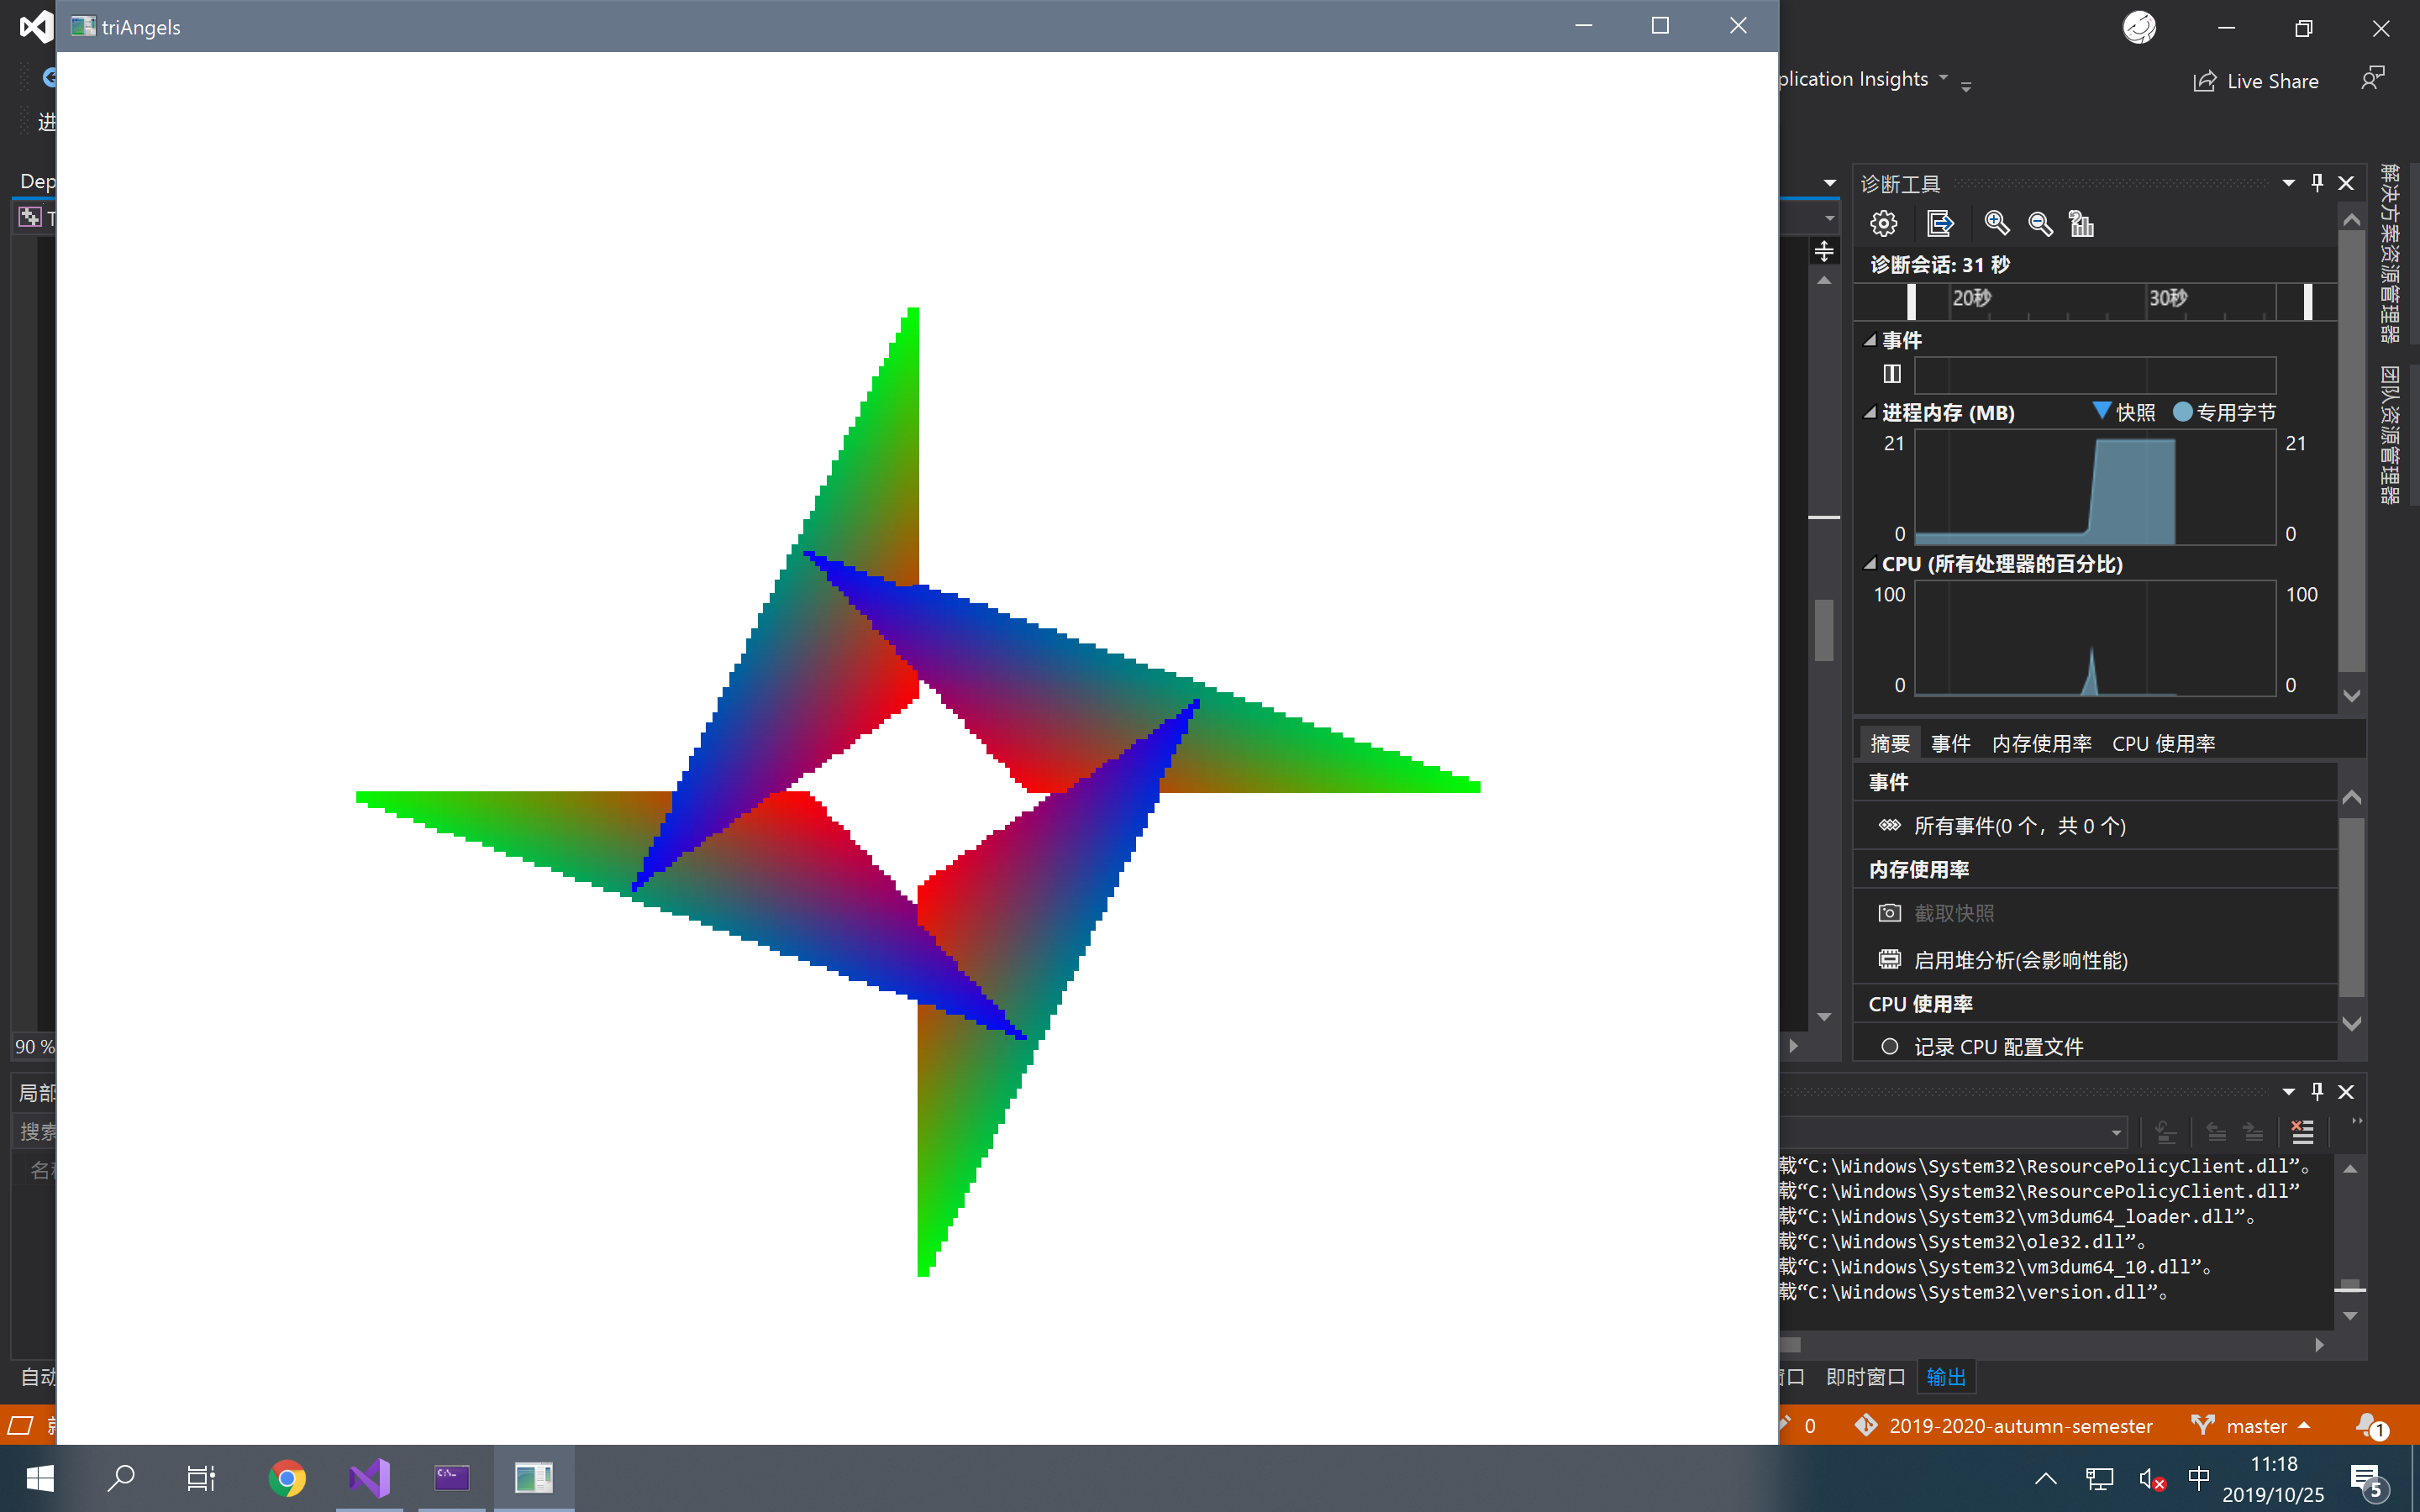
\includegraphics{/Users/yue/Documents/GitHub/2019-2020-autumn-semester/SE-344/submissions/ass2/screenshots/img.003.png}
\caption{}
\end{figure}

\begin{quote}
「\texttt{overlapping.tri}」的渲染结果,使用自定义的扫描线算法
\end{quote}

\begin{figure}
\centering
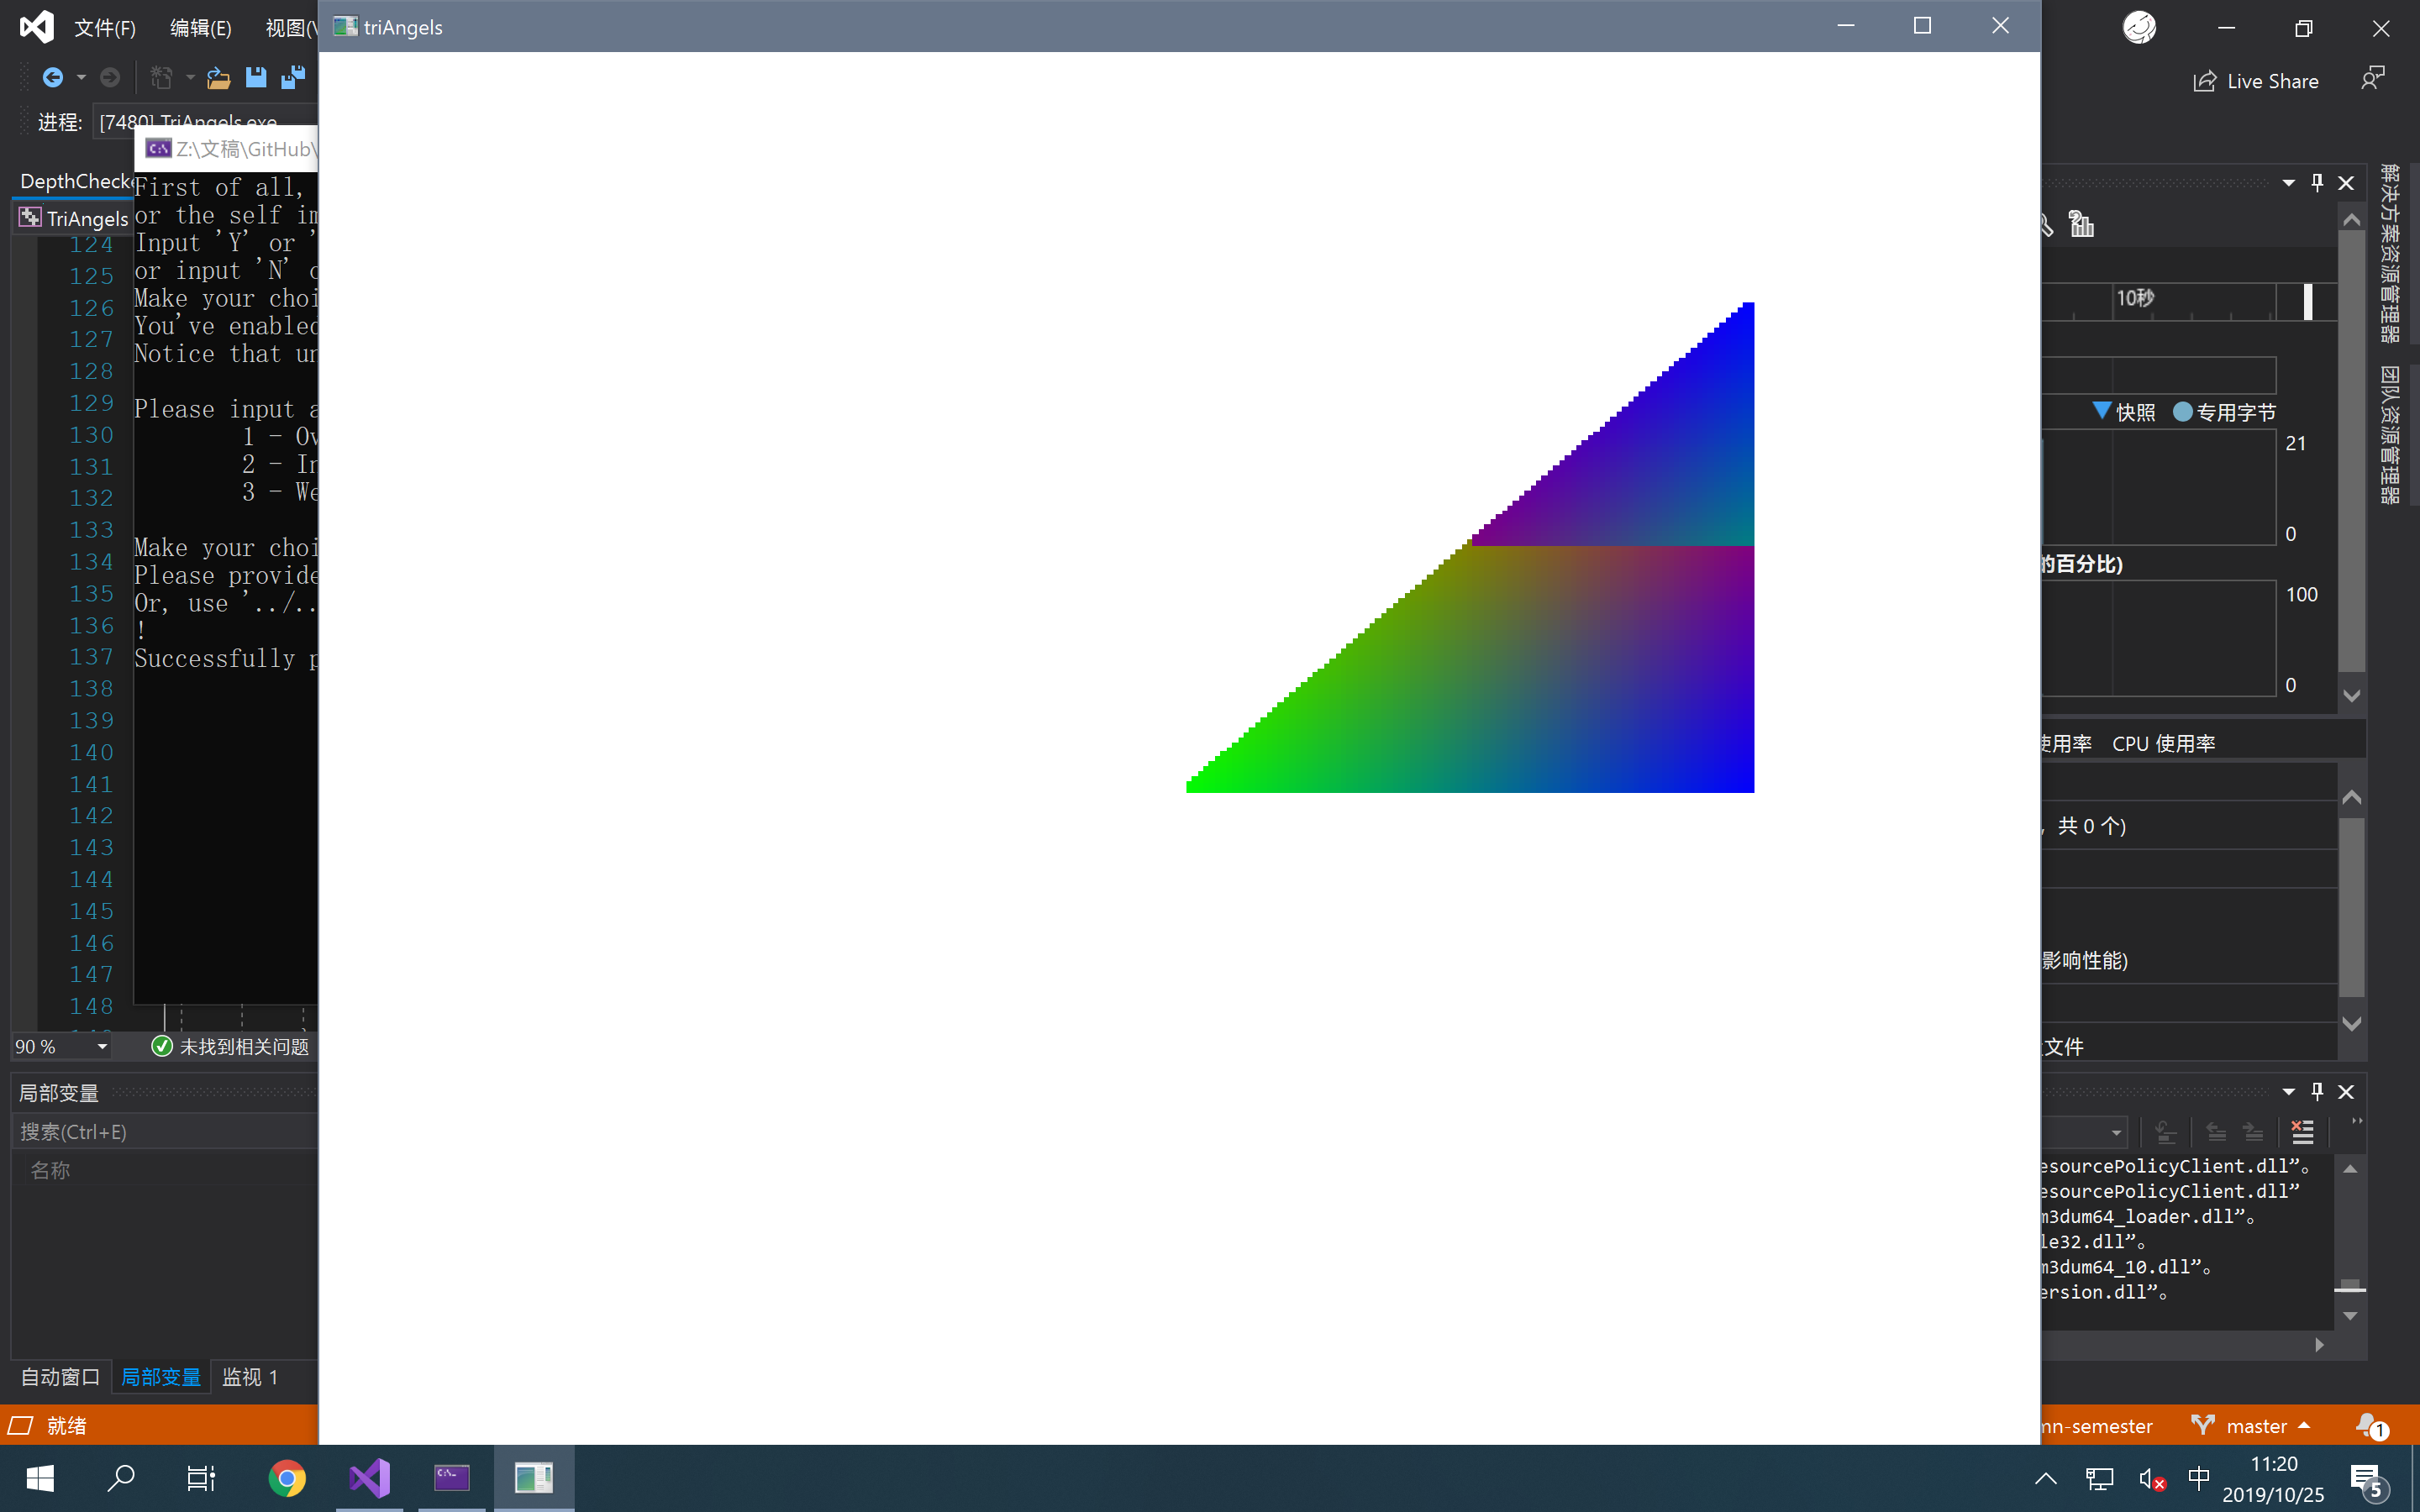
\includegraphics{/Users/yue/Documents/GitHub/2019-2020-autumn-semester/SE-344/submissions/ass2/screenshots/img.004.png}
\caption{}
\end{figure}

\begin{quote}
「\texttt{intersecting.tri}」的渲染结果,使用自定义的扫描线算法
\end{quote}

\begin{quote}
⚠️
留意到由于视角问题,两个三角形略有重合。但是从三角形中点连线的颜色突变可以看出
Intersecting 效果。
\end{quote}

\hypertarget{header-n343}{%
\paragraph{第五部分:矩形编织}\label{header-n343}}

此部分相对于上面的算法没有特别之处。为了实现编织效果,这里采用的方式是模拟真实世界中的编织方式,令水平方向的条带始终维持在
\(xOy\) 平面上(即 \(z = 0\)),而令竖直方向的条带深度在 \(-1\) 和 \(1\)
之间摇摆,以实现类似于实际的编织效果。

\hypertarget{header-n347}{%
\subparagraph{程序结构}\label{header-n347}}

相关文件包括 \texttt{Weaving.hpp},其中的 \texttt{Weaving}
类可以生成实现矩形编织效果的三角形数组。

其主要逻辑为在一个 for
循环内反复生成三角形所构成的四边形,连接成条带状。

为了体现渲染器的普适性,将不对上面的渲染算法做任何更改。

\hypertarget{header-n358}{%
\subparagraph{优化效能}\label{header-n358}}

由于这里的所有连续条带都是单色的(不存在颜色渐变问题),因此在栅格化方法内提供一个单色模式,在此时不去计算颜色插值,而直接采用提供的单色来提高效率。

\hypertarget{header-n363}{%
\subparagraph{观察结果}\label{header-n363}}

\begin{figure}
\centering
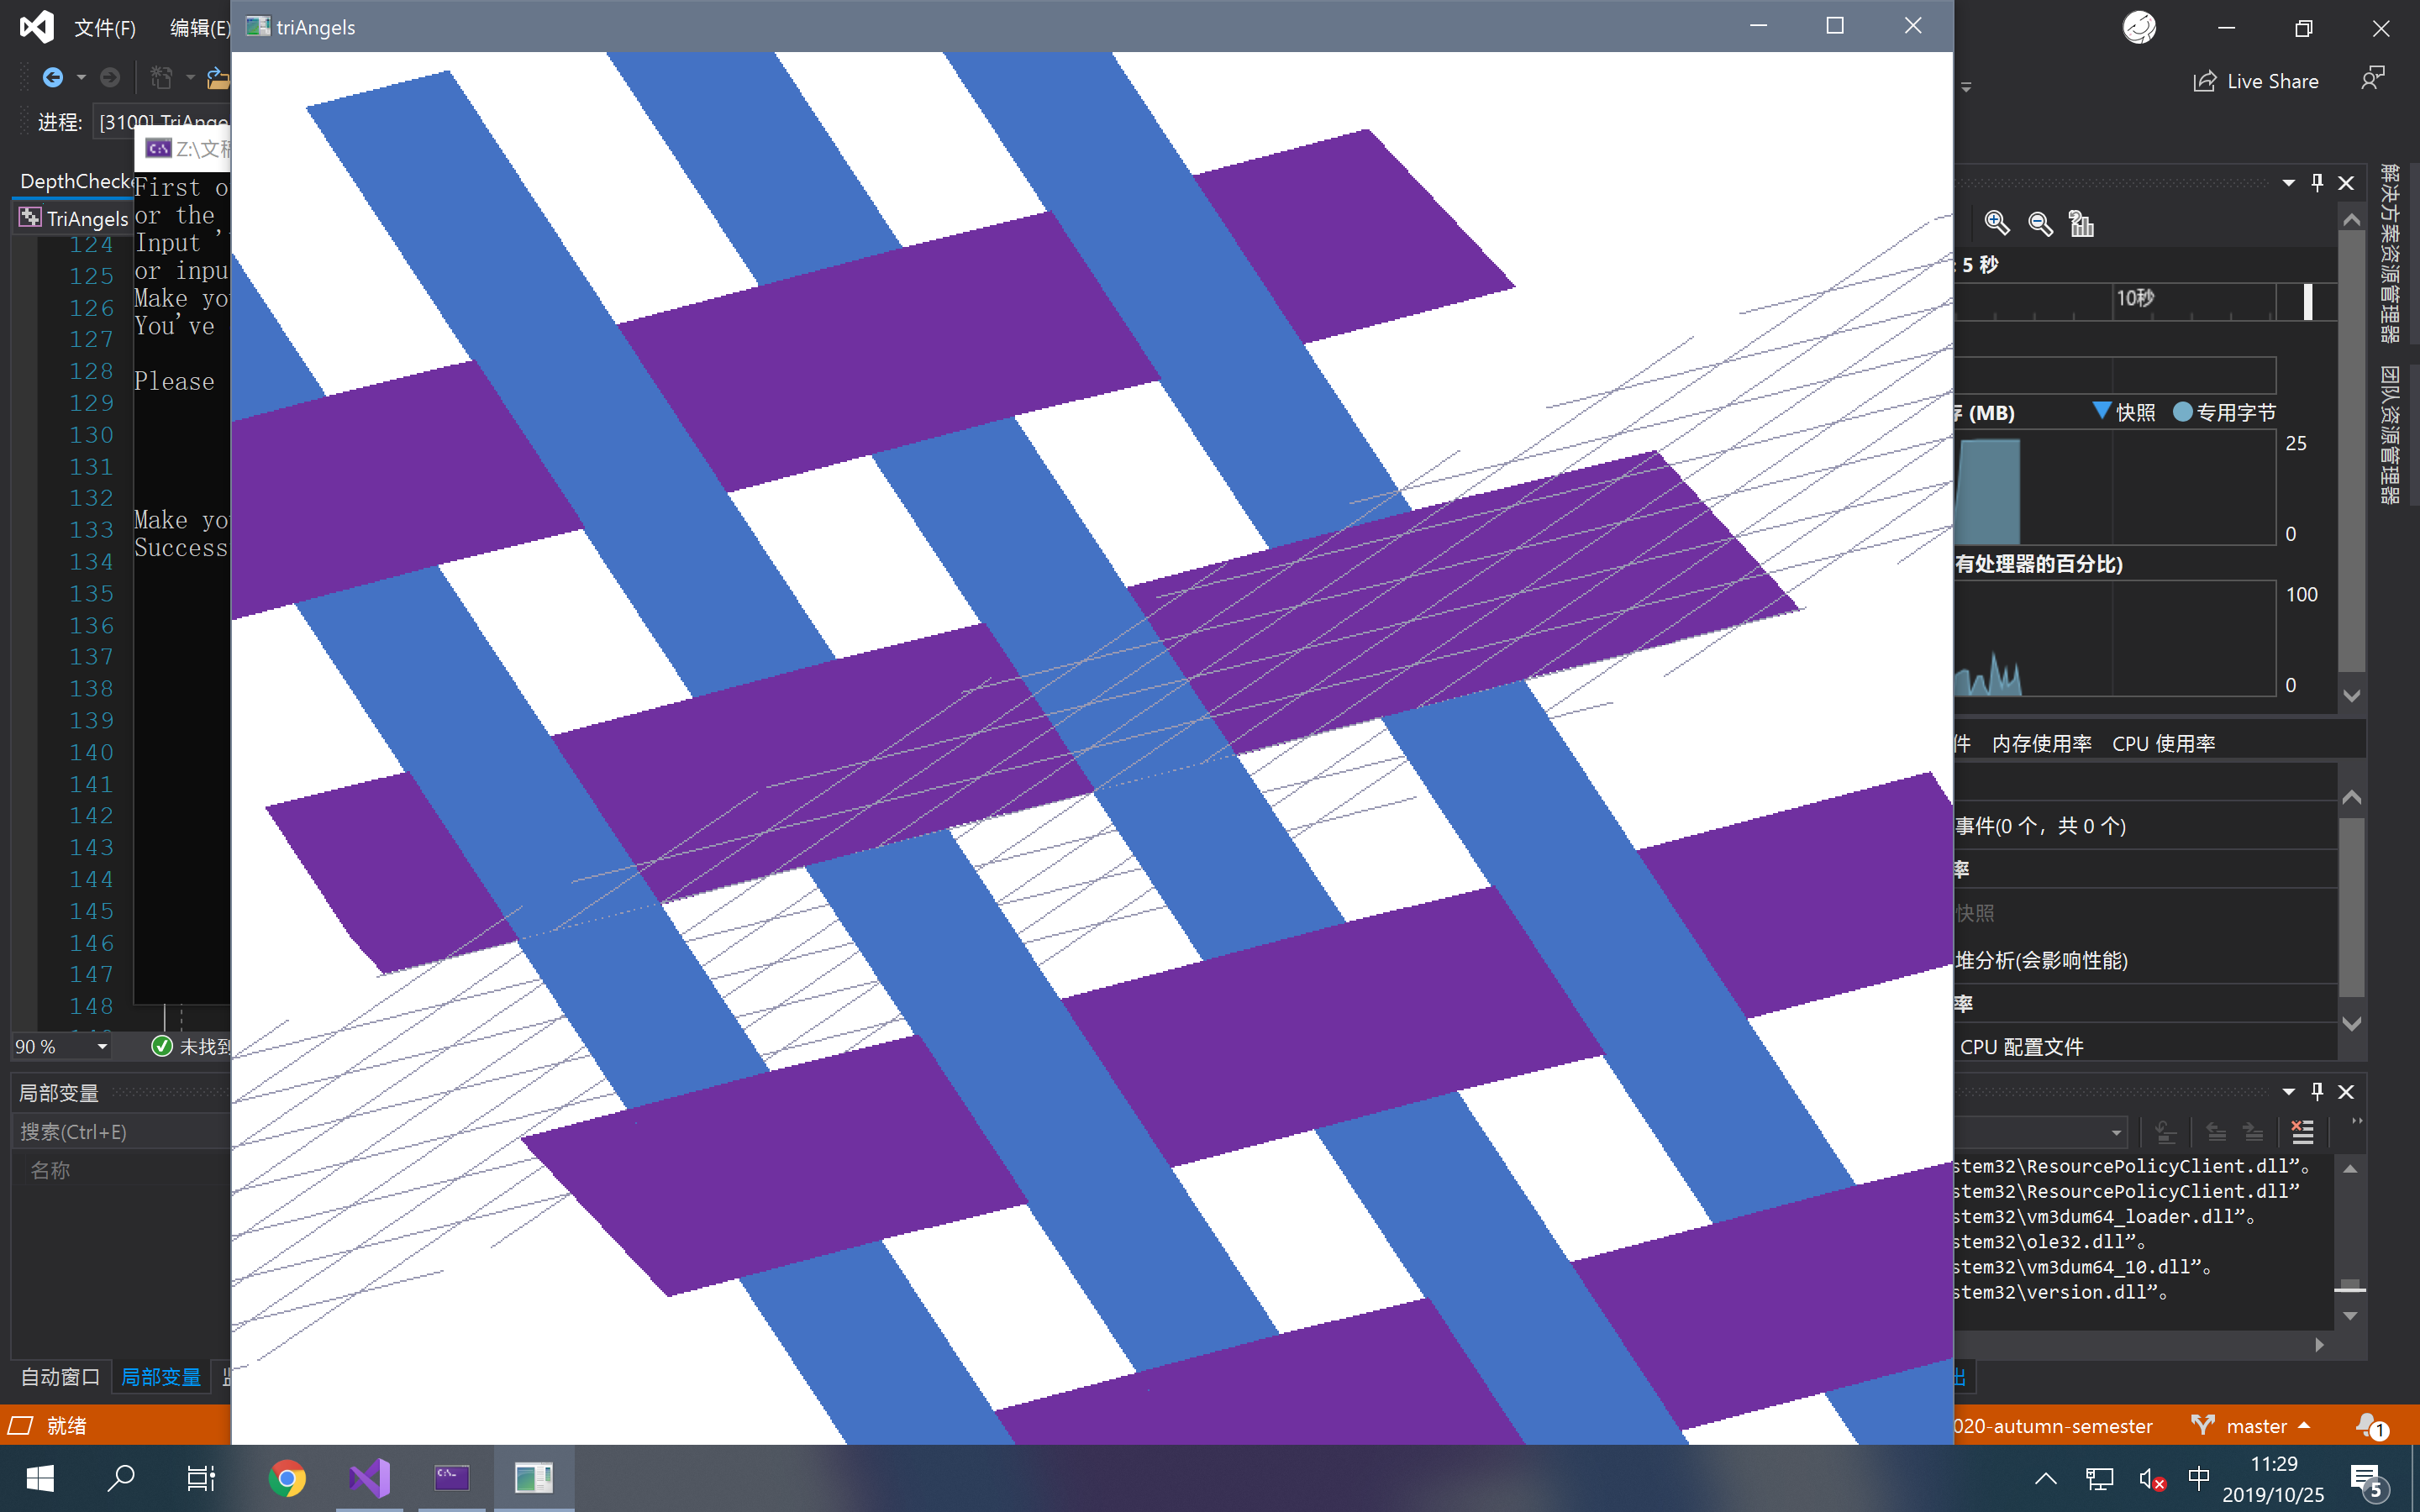
\includegraphics{/Users/yue/Documents/GitHub/2019-2020-autumn-semester/SE-344/submissions/ass2/screenshots/img.005.png}
\caption{}
\end{figure}

\begin{quote}
矩形编织效果,使用随附的深度检测算法
\end{quote}

\begin{figure}
\centering
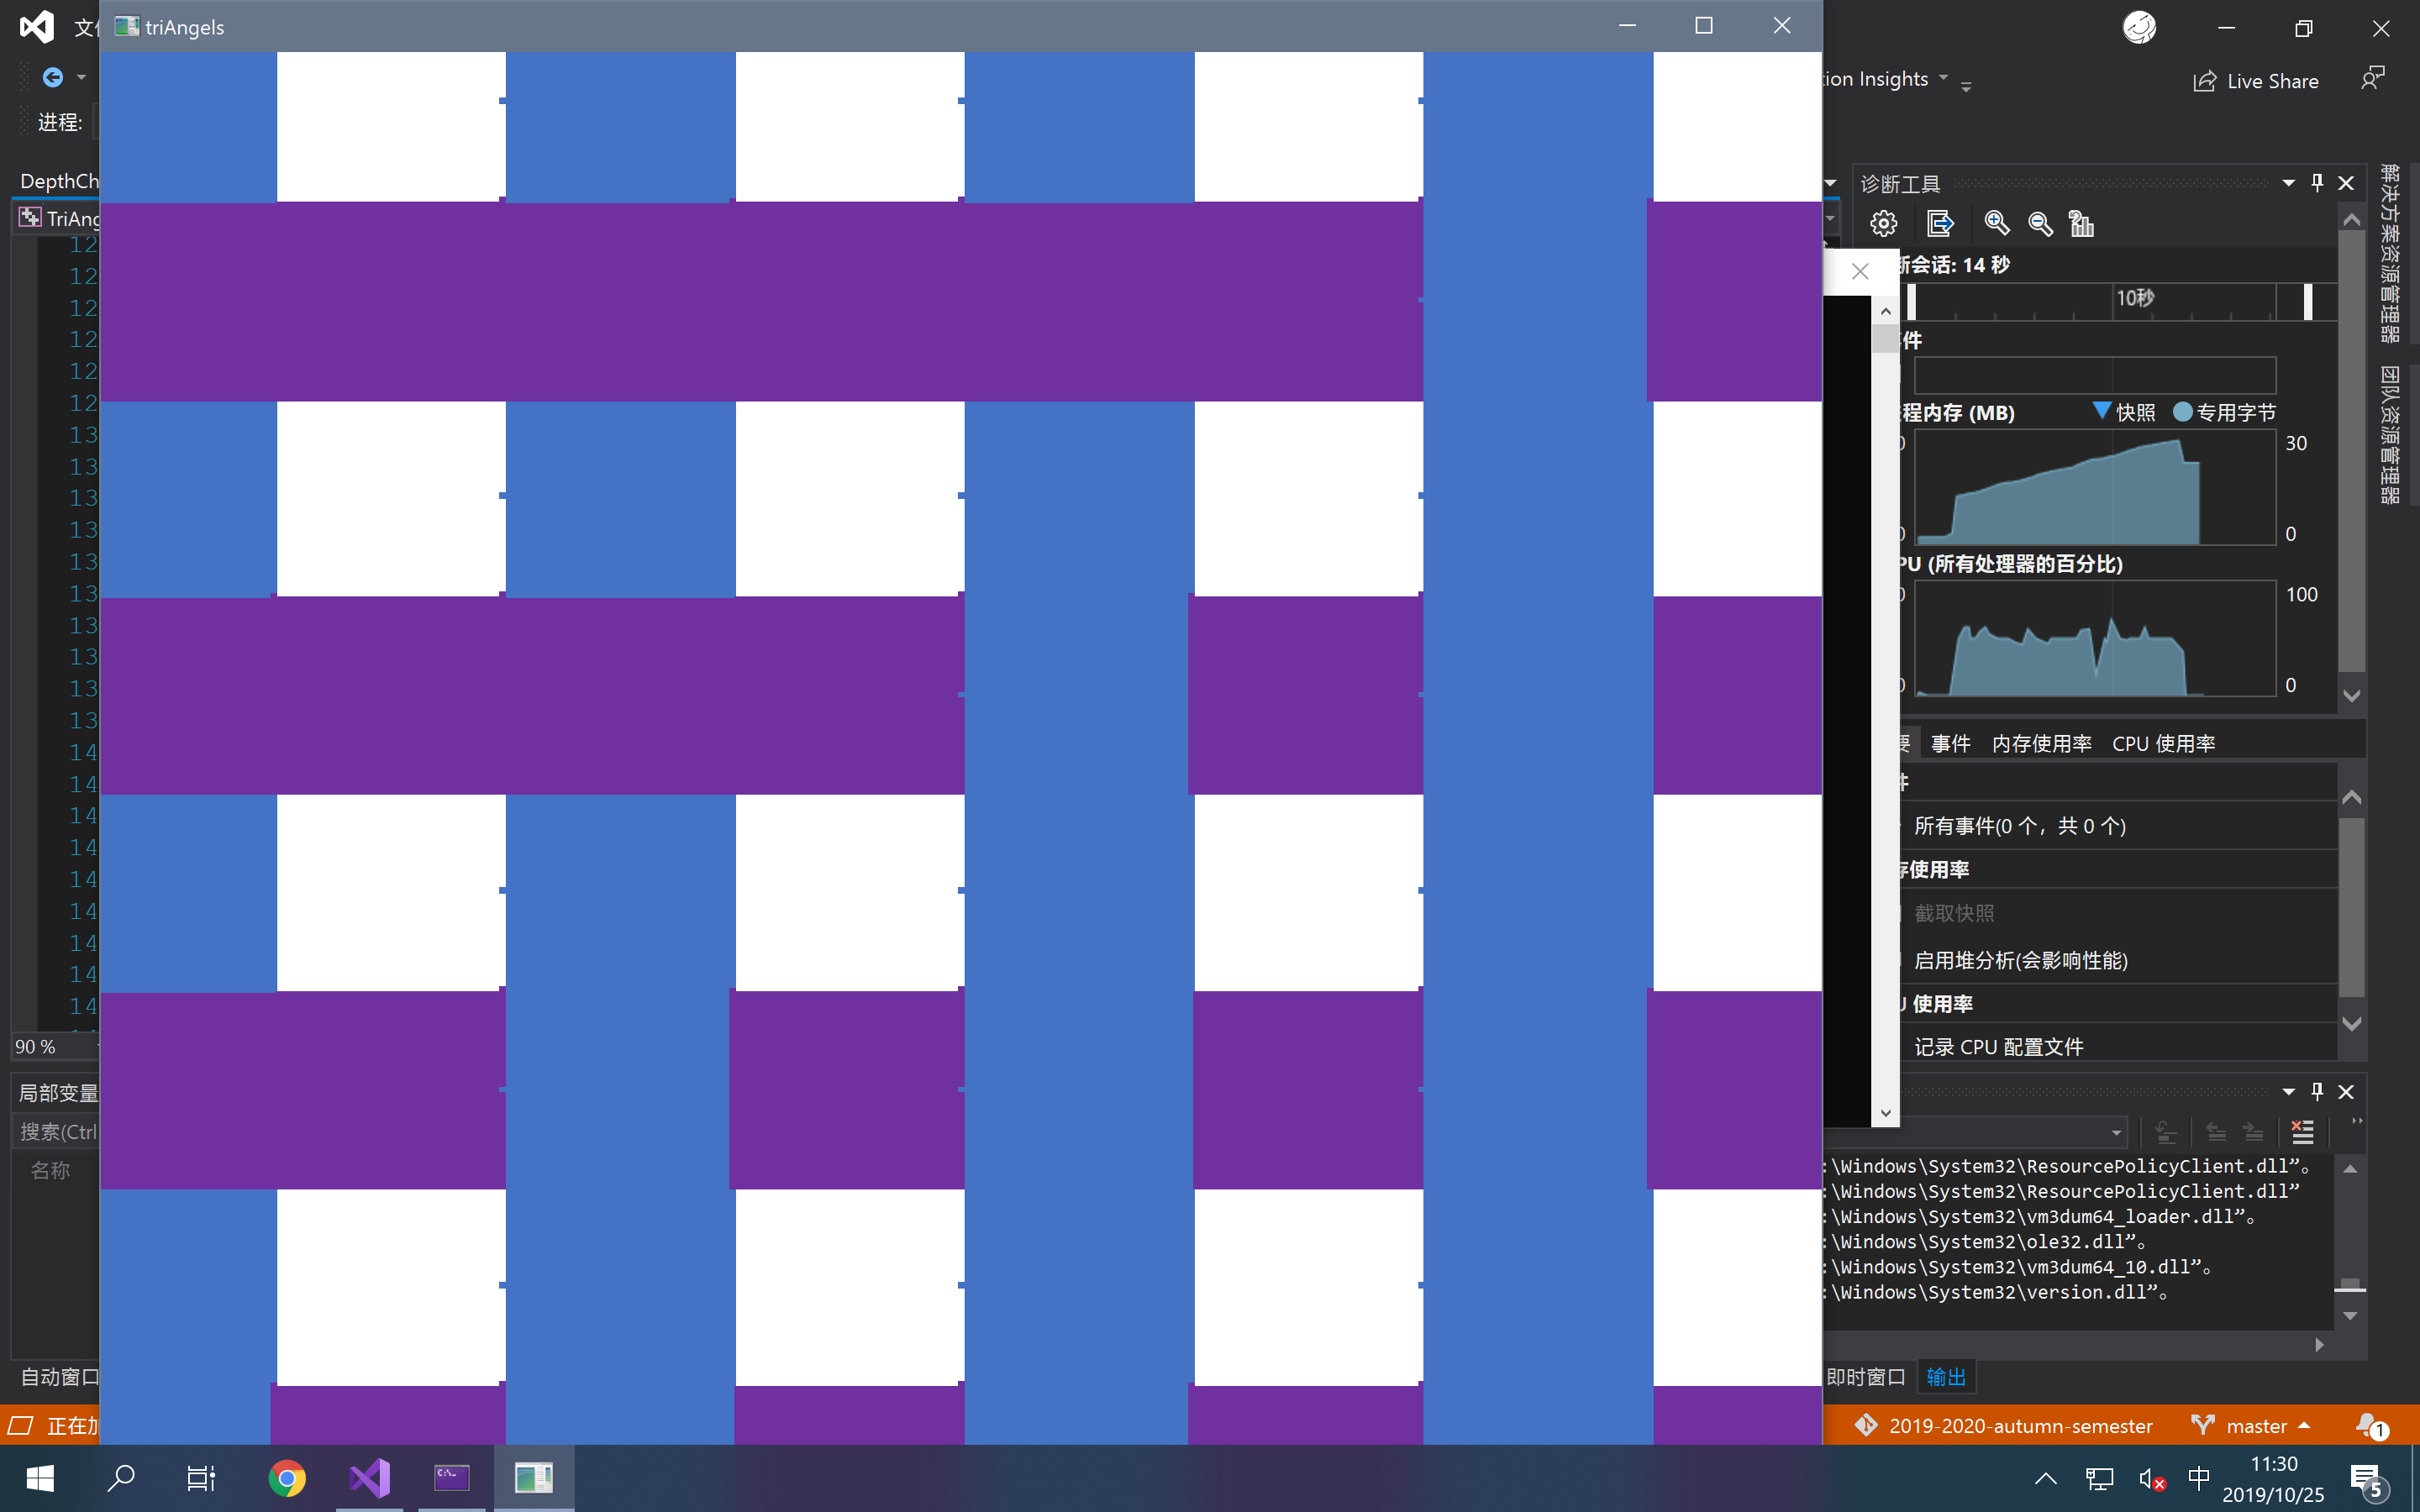
\includegraphics{/Users/yue/Documents/GitHub/2019-2020-autumn-semester/SE-344/submissions/ass2/screenshots/img.006.png}
\caption{}
\end{figure}

\begin{quote}
矩形编织效果,使用自定义的扫描线算法
\end{quote}

\begin{quote}
⚠️
注意:由于需要绘制的三角形较多,使用自定义扫描线方法渲染较慢,开启优化后在测试机器上大约需要
5 至 10 秒完成渲染。请耐心等待。
\end{quote}

\end{document}
